\documentclass{standalone}


\usepackage{fontspec}
\usepackage{sunpath}
\usetikzlibrary{hobby}

\usepackage{hyperref}

\pagecolor{white}
\begin{document}
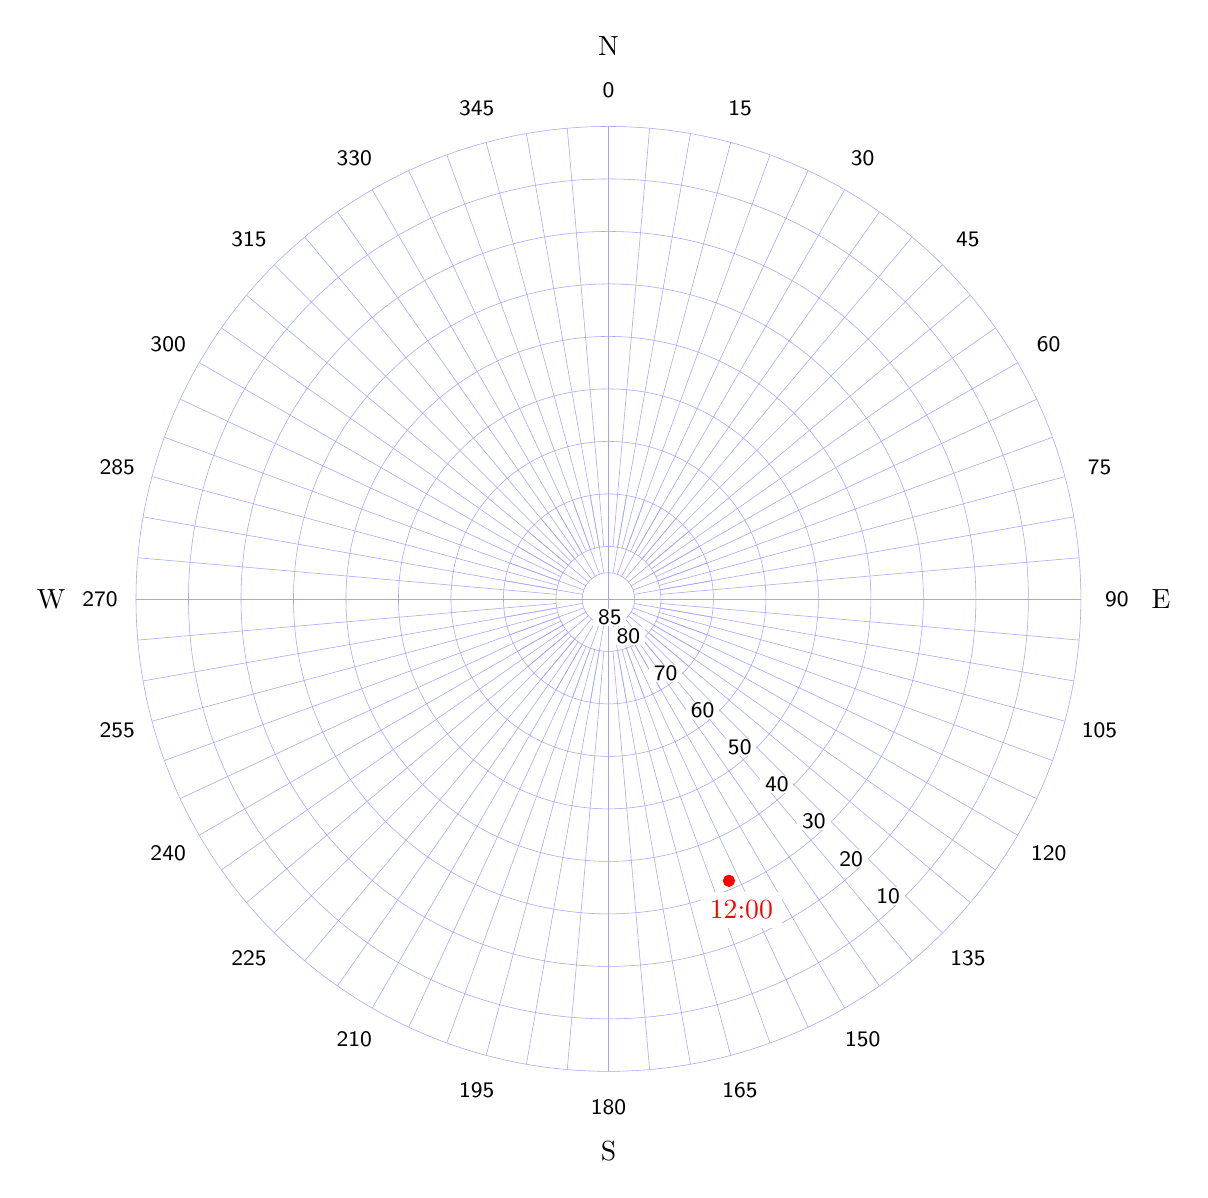
\begin{tikzpicture}[spradius=6,altitude mapping=equidistance]
\tikzset{
  sun path curve/.style={draw=red!20,thick},
  sun point/.style={radius=2pt,draw=red,fill=red},  
  sun label/.style={below,fill=white,outer sep=4pt,text=red},
}
\spcrosshair
\spaltitudecircle{{0,10,...,80,85}}
\spazimuthline{{0,10,...,360}}{85}{70}
\spazimuthline{{0,5,...,360}}{80}{0}
\spzimuthtick


\coordinate (P3) at (sunpath cs:azi=156.854847,alt=31.593335);

\path[sun point] (P3) circle;

\node[sun label,anchor=270-156.854847] at (P3) {12:00};

\spaltitudelabel{{10,20,...,80,85}}
\spazimuthlabel{{0,15,...,350}}
\spgeodirection
\end{tikzpicture}
\end{document}

